
\chapter{Introduction}

The following bachelor thesis is part of the "Ask your Repository!" bachelor project.\footnote{\url{https://hpi.de/giese/lehre/bachelorprojekte/ask-your-repository.html}}\\
In this thesis, I will demonstrate a possible solution for the issue of synchronizing development on voice interfaces with that of application code by checking voice interface configuration into version control alongside the code it corresponds to. The focus will be on allowing the use of version control for Voice Interface configurations.\\
To approach this goal, I have designed a Domain Specific Language (DSL) to describe the configuration of a voice interface in a text-based but still abstract and intuitive way. \\
I will focus on development using Google Dialogflow as it is the most widely used tool; it is also what my bachelor team is using in our project. \citeNeeded

I propose that by designing a DSL that can be used to configure a Dialogflow agent in a way that is text based and can be managed by version control systems like Git - but that still feels seamless to a user and is intuitive to use for a developer familiar with the Dialogflow web interface - development on voice interfaces can be simplified and development teams in the future will be able to work on voice assistants in the same way that they are used to working with code. This opens up the entirety of code based tools which exist for making development more streamlined for the development of voice interfaces, while keeping the robustness of code which can be saved in version control.

In chapter 2, I will explain the current situation in regard to voice interface technology and version control. Afterwards, in Chapter 3, I will then more closely examine the main problem caused by the given situation.
Chapter 4 will focus on finding a solution to the above mentioned problem, and on the specific solution, I built a prototype for. Going into more detail, chapter 4.2 will show how I used Xtext to create a grammar and code generator for configuring Google Dialogflow agents. This grammar was used to provide syntax highlighting and validation in Eclipse DSL; the output of the code generator is a valid voice interface configuration in its JSON representation, ready to be imported into Google Dialogflow.
Lastly in chapter 5, I will evaluate the sucess of the prototype by comparing it to an alternative way of checking voice interfaces into source control. 

\chapter{Status Quo}
\section{Voice Interfaces}
Voice assistants and voice interfaces are increasingly popular technologies that are experimented with and used by every major player in the technology market \citeNeeded. To keep up with this trend, developers either need to be able to build their own voice interfaces or integrate with an existing system of which Google Assistant and Amazon Alexa are the most relevant. \citeNeeded
Currently, depending on whether you are developing for Google Assistant or Alexa, designing a voice interface for one of these systems usually entails working with either Google Dialogflow or Amazon Lex. These are powerful tools which enable developers or domain specialists to quickly and easily design a voice interface.
These tools are interacted with through a website which provides a graphical editor for the configuration of the voice interface. Although this makes the initial development of a voice interface easier, it comes with a severe drawback.

\section{Version Control}
While the web interface makes initial setup of the voice interface easier for a single domain expert or developer, new difficulties arise when a team of developers is working on a voice interface in an iterative fashion. It becomes crucial for the team to manage versions and track changes to the interface along with the changes to the application the interface is supporting. \citeNeeded

The state of the art solution for managing iterative work in development teams is Git. \citeNeeded
Git provides a functionality for saving snapshots of specific iteration in your project and handling the problems that come up in iterative work.
These problems are:
\begin{itemize}
    \item merging work done by multiple users
    \item ensuring that a stable version of a project is saved while developers are working on more experimental changes
    \item giving the team the ability to easily track and revert changes that have been made.
\end{itemize}
The issue that arises is that the above mentioned technologies are not compatible and the configuration of a voice interface can easily get out of sync with the changes made to the application and managed in Git. \citeNeeded

\section{Previous Work}
Previously, similar issues have been solved for other technologies \citeNeeded (cite this, evtl the Evolution control paper or with smt. from here \url{https://scholar.google.de/scholar?hl=de&as_sdt=0%2C5&q=version+control+xml&btnG=})  by designing Version control systems that specialize in managing the artifacts those technologies rely on. 

\section{Lack of Solution}
A solution like this has not been built for Dialogflow, most likely because voice interface tools like Amazon Lex or Google Dialogflow are a newer development, with Dialogflow having only existed in its current fashion since October 2017 \citeNeeded and the Dialogflow V2 API that I am using, and that was necessary for the success of this project is currently in Beta stage. The V2 API is generally available since 17 April 2018
(\url{https://blog.dialogflow.com/post/v2-and-enterprise-edition-generally-available/}  4.6.2019)
And “V1 of Dialogflow´s API will be deprecated on October 23, 2019”. (\url{https://dialogflow.com/docs/reference/v1-v2-migration-guide} , 4.6.2019).
Dialogflow is currently still transitioning tot he use oft he new V2 API.
It is the V2 API that makes this project possible because it includes the agent management APIs used for exporting, importing, and updating of Dialogflow "agents" (this is what Google calls a specific voice interface) using the JSON format.

\chapter{Problem Statement}

As stated before, currently there is no version control system for Dialogflow agents.
This is problematic because when designing a voice interface, it is necessary to make iterative changes, so the voice interface can evolve alongside the application it supports. This can lead to issues in the following workflows that are common in software development:  (Reword this to prepare for ALL points below)
\begin{itemize}
    \item When starting work on a new feature a new branch is created. This is done so that changes, which might not work right away, are contained to this branch and can be merged into the main application at a later time. If this feature requires changes to the voice interface, a problem may arise, because the voice interface has no mechanism for branching.
    \item Once experimental changes on a feature branch advance to a point where they are meant to be included in the master branch, code can simply be merged from one branch to another. The changes to a voice interface configuration cannot be included in a pull request.
    \item When working on a product it is generally considered to be “best practice” to have code that should be merged into the master branch from a feature branch reviewed by at least one or two other developers to make sure that it is working as expected and does not have any obvious flaws. This cannot be done for changes to a voice interface.
    \item When working in a team, it is not always possible to remain aware of all the changes team members have made. Source code that is managed in Git automatically creates a history of all changes, which is highly valuable to the developers. This type of history does not exist for the voice interface configuration.
    \item Open source development is an important part of today's development landscape. Since voice interfaces are not usually checked into source control alongside application code, open source development of voice interfaces or applications that use voice interfaces is stifled. In addition, open source projects can be forked by other developers and can be improved by many developers in an iterative fashion. This is another advantage that voice interfaces are currently lacking. \\
          When working on a Dialogflow agent, one can save a version of the configuration and then continue as a draft, but Dialogflow assumes that you will only ever have one draft at a time. Versions are also designed in a linear fashion with no way to merge changes from multiple versions. This is obviously nowhere near the depth of features that are necessary in version control and all of these features are already provided for normal code by using the current state of the art version control system, Git.
\end{itemize}

In summary the problem is that there is no sufficient version control system that is compatible with Dialogflow.

\chapter{Approach}

\section{Choosing a Direction}

\subsection{Version Control System}

Since there is no version control system that is compatible with Dialogflow the obvious solution might be to build a new version control system that is compatible with Dialogflow. This has been done before for other technologies (cite this, evtl the Evolution control paper or with smt. from here \url{https://scholar.google.de/scholar?hl=de&as_sdt=0%2C5&q=version+control+xml&btnG=}) but I decided against this approach for multiple reasons.

Firstly, I believe that it will be hard to get developers to move from an established tool like Git; I assume that developers would not choose to give up feature rich support that exists for Git (Github, Gitlab, Bitbucket to only name a few).
Secondly, using a specific version control system that is developed to allow compatibility with Dialogflow, it would be hard to also maintain compatibility with other tools.

Therefore, instead of trying and failing to develop a competing standard to Git, I decided to make use of a workaround that is possible with Dialogflow.

\subsection{Git with exported JSON files}

It is possible to export a folder with a JSON representation of an agent and save this in Git. This solves some of the issues mentioned in chapter X (…), but an agent's JSON representation is not intended for readability by humans, and neither is it meant for direct editing. This makes certain aspects of the workflows I described above much harder, e.g. conducting a code review, since it is difficult to read the changes to the JSON files describing the agent’s configuration.

\subsection{Domain Specific Language}
While trying to solve the problems mentioned so far, it became obvious that a solution to these problems would require configuring an agent in a format that is compatible with text based tools like Git but that also maintains or even enhances upon the maintainability and readability of Google Dialogflow configuration in the web interface.
For this purpose, I designed a domain specific language (DSL) in order to create a text-based notation (DSL code) for the configuration of an agent.


\section{DSL Engineering}


\subsection{WHAT IS A DSL}
REPLACE THIS\\
The DSL consists of 2 main parts.
Firstly, there´s a grammar which defines what you can write in the DSL.
The grammar contains all possible combinations of words that you can use to write in this language
Specifying this grammar allows me to have live IDE support including syntax validation while writing DSL code. Which Markus Voelter says is a vital part of DSL design. \citeNeeded (cite this using Markus Voelter: dsl engineering)

The other part I built is a code generator.
What this does is it takes input in the form of code that is written in a DSL in accordance with the grammar, and output files containing generated code,
In this case containing the full JSON representation of a Dialogflow agent.

On a higher level, let´s have a look at this graphic: …

\subsection{Requirenments for the DSL}

In order to provide a tangible benefit the DSL must fulfill a number of requirements:
\begin{itemize}
    \item It needs to be significantly shorter than the JSON representation of an agent.
    \item It needs to be more readable than the JSON representation.
    \item It needs to create smaller diffs (sum of changed lines) than the JSON representation when making changes.
    \item A user needs to be able to automatically compile and update an agent on the web from DSL code.
\end{itemize}

During the process of my work it became clear that solving the above mentioned problems made it necessary to find solutions for every one of these requirements.

\subsection{Design Decisions}

I wanted the DSL code to read naturally for a developer used to the Dialogflow interface.
In order to achieve this, I tried to closely mimic the structure of the web interface in my DSL code.

In order to show this, I will walk you through an example agent I created for testing purposes. The agent is a very simple controler for regulating the air conditioning in a room. It listens to the user and sends their requests to a server. Throughout the four steps of this example, I will follow a pattern of first showing how a developer would set up an agent on the Dialogflow website, followed by showing how to do the same in DSL code.

\subsubsection{Creating an Agent}
First a developer needs to create a new agent. To do so, they click on "create agent", and enter the agent's name and language as seen in \autoref{CreateAgent}.
To achieve the same effect, in DSL code, a developer would enter the following:

\begin{verbatim}
    Agent TestAgent_RoomTemperature
        language en 
\end{verbatim}

\begin{figure}[ht]
    \centering
    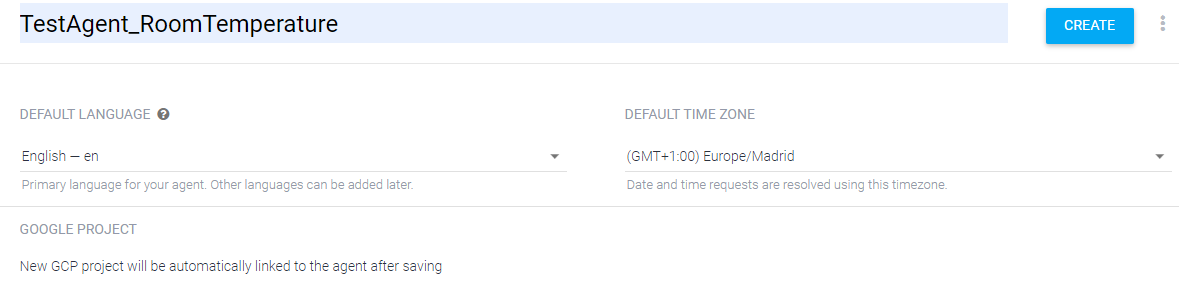
\includegraphics[width=1\textwidth]{Thesis Images/CreateAgent.PNG}
    \caption{Creating an agent on Dialogflow.}
        \label{CreateAgent}
\end{figure}

\subsubsection{Setting an Entity-Type}
In the next step, an entity-type needs to be created to allow to intuitively turn on and off the air conditioning.
In Dialogflow this is achieved by filling in the form seen in \autoref{CreateType}.
In DSL code the same can be done by writing the following:

\begin{verbatim}
    Agent TestAgent_RoomTemperature
        language en 
    
        Type ACState
            values 
                "On" ("Active" "Enabled" "On"),
                "Off" ("Inactive" "Disabled" "Off")
        auto_expand
\end{verbatim}

\begin{figure}[ht]
    \centering
    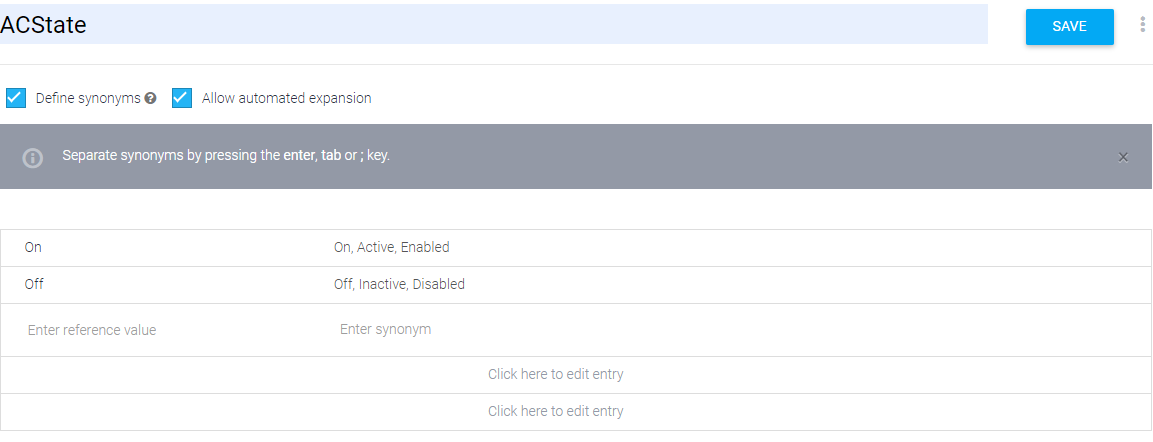
\includegraphics[width=1\textwidth]{Thesis Images/CreateType.PNG}
    \caption{Creating an entity-type on Dialogflow.}
        \label{CreateType}
\end{figure}

\subsubsection{Setting a Webhook}
For the agent to actually affect an air conditioner in the real world, it needs to send the user's request to a webserver. To do so, a webhook is enabled in Dialogflow by filling in the form as seen in \autoref{CreateWebhook}.
In DSL code the same can be achieved:
\begin{verbatim}
    Agent TestAgent_RoomTemperature
        language en 
            
        Webhook 
            active 
            url "https://fake.ac_controller.com/vi_webhook"

        Type ACState
            values 
                "Off" ("Inactive" "Disabled" "Off"),
                "On" ("Active" "Enabled" "On")
        auto_expand
\end{verbatim}

\begin{figure}[ht]
    \centering
    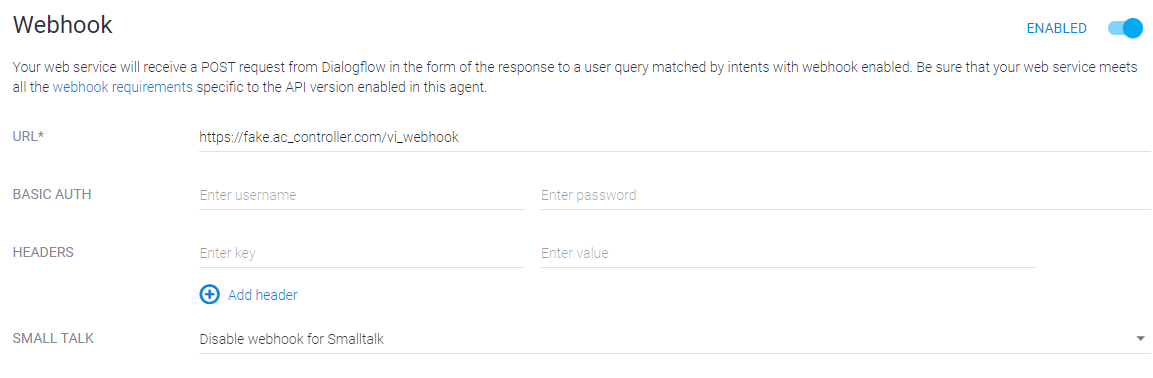
\includegraphics[width=1\textwidth]{Thesis Images/CreateWebhook.PNG}
    \caption{Setting a webhook on Dialogflow.}
        \label{CreateWebhook}
\end{figure}

\subsubsection{Writing an Intent}
The last and most vital step is to create an intent that the agent can understand. This is done on the website by filling in the form seen in \autoref{CreateIntent} and can alternatively be achieved in DSL code as follows:
\begin{verbatim}
    Agent TestAgent_RoomTemperature
        language en 
            
        Webhook 
            active 
            url "https://fake.ac_controller.com/vi_webhook"

        Type ACState
            values 
                "Off" ("Inactive" "Disabled" "Off"),
                "On" ("Active" "Enabled" "On")
        auto_expand

        Intent SwitchAC
            parameters
                state ACState (required prompts "Did you want the AC turned On or Off?")
            trained with phrase
                "Turn" state "the AC",
                "Set the AC to" state,
                "Set the air conditioner to" state,
                "I want the AC turned" state,
                "Make sure the AC is" state
            webhook_fullfillment
\end{verbatim}

\begin{figure}[ht]
    \centering
    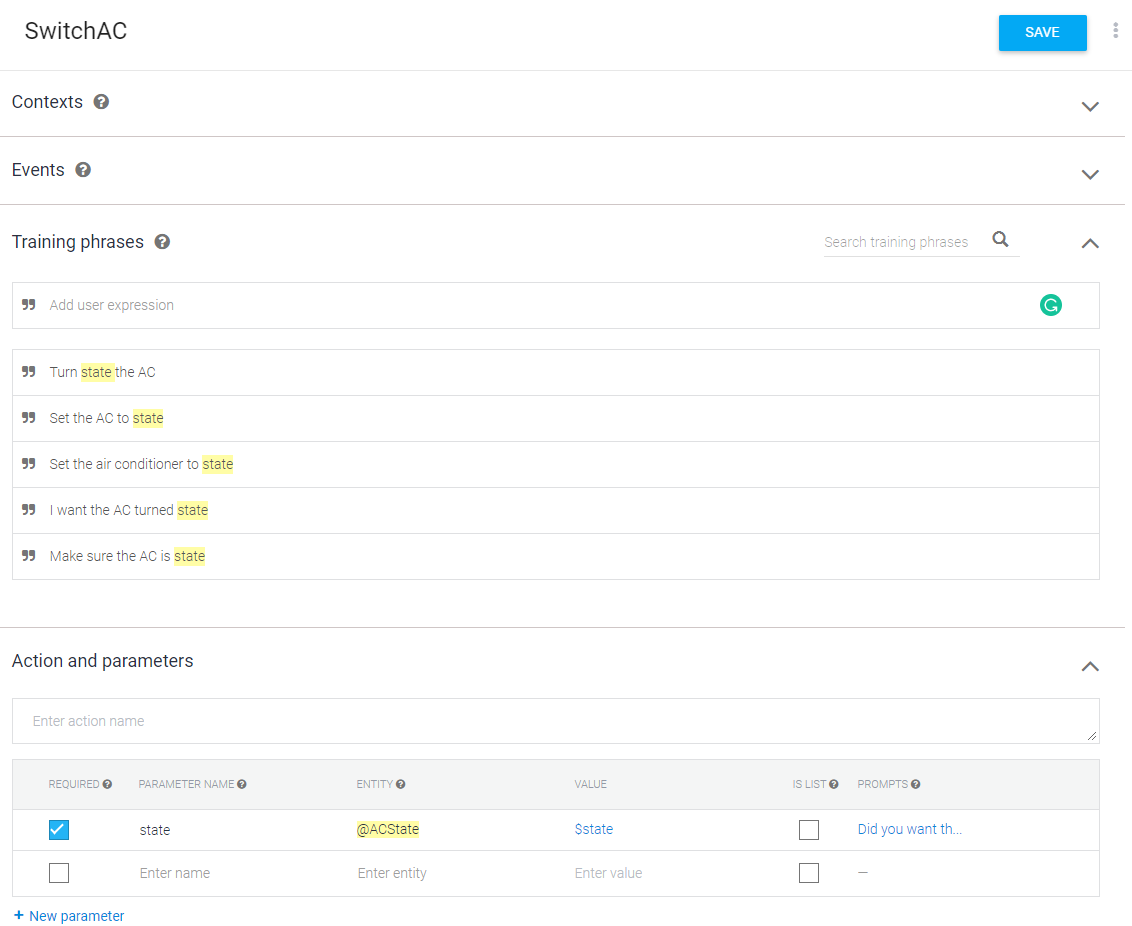
\includegraphics[width=1\textwidth]{Thesis Images/CreateIntent.PNG}
    \caption{Setting up an intent on Dialogflow.}
        \label{CreateIntent}
\end{figure}

\subsubsection{Summary}
From the above it becomes apparent that the DSL I designed is a viable alternative to using the Web interface.
From personal expirience I can say, that I can configure an agent more quickly in the DSL code than in the Web interface. However in the following section of this chapter, I will talk about which conseccions I had to make and which disadvantages the DSL still has to overcome, for some of which I will offer solutions.

\subsection{Concessions and Drawbacks}
UNFINISHED

The parameters are entered before training phrases to allow for validation of training phrases that use these parameters.

Problem: Changes to DSL code are not affected by dynamic entity changes via API.
Next it is possible to enter either the keyword “dynamic” or the keyword “values” followed by a comma separated list of values that are possible for this type.
This allows the user to either enter a type with it’s associated values, or have the type exist in the DSL and be valid for validation - but not have any JSON files generated for it, so as not to overwrite an entity type that is dynamically set on Df via the API.
This is relevant in cases like the team selection in our Ask your Repository project.
In that case a list of teams was kept as an entity type, and dynamically updated whenever new teams were created. This allowed the user to say “Select Team” followed by their team’s name and have the voice interface understand their team name.

\subsection{Usage}
When you use the tool/compiler that I built, you run this compiler with the input being the DSL code; the output will be a full JSON representation of a Dialogflow agent which can be sent to the Dialogflow V2API.
The V2API allows you to update the online version of your agent using the JSON files.


\section{Circumstances under which using the DSL is beneficial}
Under which circumstances will the DSL provide a benefit for a project?


\chapter{Evaluation}
In the following chapter I will evaluate the performance of my DSL-prototype.
Testing and evaluation has been done by myself by referring back to the requirements I stated earlier in chapter four. A future larger scale survey would be welcome but was not part of this evaluation.\\
The requirements I used for evaluation were:
\begin{itemize}
    \item Length
    \item Readability
    \item Diff size
    \item Automatic compilation and update
\end{itemize}

In the following sections I will talk about each of these requirements and whether and in howfar my prototype can fulfill them.

\section{Length}

In order to provide a tangible benefit the DSL code must be significantly shorter than the JSON representation. Coming back to the agent used in chapter four, I can show that the DSL code for that agent is exactly 23 lines long, while using a large amount of whitespace and linebreaks to support readability.

The JSON version for this same agent, however, comes in at exactly 200 lines as you can see in the appendix. \ref{}REFTHISLATER \url{https://github.com/arne-z/BachelorThesis/commit/d61614158d41d72bb72f28f941718a707d72a5e0}

CREATE MORE TESTCASES. REFER TO THEM HERE. PUT IN APENDIX.

TABLE!!!


This demonstrates, that the DSL code for an agent is significantly shorter than the JSON version. Less code causes better maintainability and faster and easier code reviews. 

\section{Readability}
In order to provide a tangible benefit the DSL code must be more readable than the JSON representation.
\citeNeeded Definition of readability == undefined



\section{Diff size}
In order to provide a tangible benefit the DSL code must create smaller diffs (sum of changed lines) than the JSON representation when making changes.

Using the air conditioning example again, when making a change - in this case adding more training phrases to an agent to allow additional functionality - the diff size shows a large difference between DSL code and JSON version. In this specific example, the DSL code has a diff of 7 lines\footnote{\url{https://github.com/arne-z/BachelorThesis/commit/559f72d4dd8550d57bef8b42ee34678317e21fcb}} and the JSON version one of 124 lines.
\footnote{\url{https://github.com/arne-z/BachelorThesis/commit/08255f4b1bff5a2bb4bf57319ab37033193429c5}}



\section{Automatic compilation and update}
A developer needs to be able to automatically compile and update an agent on the web from DSL code.
The compiler created alongside this prototype\footnote{\url{https://github.com/arne-z/BachelorThesis/releases}} is able to automatically generate the JSON representation of an agent from DSL code.
Alongside this, I have written a script that automatically sends the resulting JSON files to the Dialogflow website.
This can be used in continuous integration setups like CircleCI\footnote{\url{https://circleci.com/}} to automatically keep the online version of a Dialogflow agent up to date with the most current version of the DSL code in source control.

Below you can see an example of the CircleCI job configuration that I set up for the prototype in our bachelor project.
\footnote{The full configuration set up by our bachelor project team can be found here.\\
\url{https://github.com/hpi-sam/ask-your-repository-dialogflow-adapter/blob/agent-config-with-dsl/.circleci/config.yml}}

\begin{verbatim}
    deploy_agent:
        docker:
            - image: circleci/openjdk:latest-node
        steps:
            - checkout
            - run: > 
                wget -O ./dfc_compiler.jar
                https://github.com/arne-z/BachelorThesis/releases/...
            - run: yarn install
            - run: java -jar ./dfc_compiler.jar ./Agent/Tobito.dfc
            - run: echo $GOOGLE_CERT_FILE_64 | base64 --decode > ./googleKey.json
            - run: >
                node ./utility/importAgent.js 
                --dir ./src-gen 
                --key ./googleKey.json 
                --pid projects/newagent-bdb60
\end{verbatim}

The above configuration starts a docker image with Java and Node installed - Java is required for the DSL compiler, Node for the import script - and checks out the most recent version of our project from source control.
It then downloads the DSL compiler from my github repository and runs the compiler targeting the .dfc file containing the DSL code for our project's agent.
It then runs the importAgent script that will send the JSONs generated by the compiler to the Dialogflow API.

This setup allows a "hands free" approach to developing for Dialogflow, where all the developer has to do is change the DSL code and once that is pushed to Git, the Dialogflow agent is updated automatically.


\chapter{Summary and further Work}

It was my task for this Bachelor thesis to build a prototype for Df to find out if you can configure Df agents as code in a DSL.

For further projects one could consider

•	build a second compiler for amazon lex
•	my compiler is not ready for the market (minor bugs and flaws), so there is more work here 
•	build a generator for DSL code from the JSON representation of an agent (the other way round) so you would want a “reverse compiler” to be able to input … and get, as an put, the DSL – no more manual … ! 

\chapter{Declaration of Independence}